%This is chapter 3
%%=========================================
\chapter[Method]{Materials and methods}

%In this final chapter you should sum up what you have done and which results you have got. You should also discuss your findings, and give recommendations for further work.

%%=========================================

\section{Tools and libraries}
\subsection{JavaScript}
JavaScript has mainly been chosen as the base implementation language because of its cross compatibility and popularity. ...

\subsection{Babel}
- Babel - ES6 needs to be transpiled to ES5 (Browser compatibility).
\subsection{npm}
Needed packages.. Published all packages to npm.. Most stabile compared to GitHubs new repo....

\subsection{Third party libraries}
Why did i use them???
list up like:
- xxx because ...
- xxx provides ...
Elaborate some on three.js - why is it good? (popularity)

\subsection{GitHub Actions}
Why? How did i use it? - For automation... - deeply integrated in GitHub.

\section{Working methodology}
\subsection{Scrum}
Even though this is a one man project, i have tried to adapt the scrum methodology.
...

\subsection{Requirements specification}
\subsubsection{Acceptance criteria}
Acceptance criteria - custom field in Jira.
Specially for the voxelization algorithm?

\subsection{GitFlow}
Why did i follow gitflow? Any changes to the usage?? Good for enforcing standards, automation etc..

\subsection{Semantic versioning}
All published modules are enforcing Semantic versioning. This ....

\section{three-voxel-loader}
\colorbox{green}{NEED UML DIAGRAMS}\\
The main goal for the three-voxel-loader is to generate a 3D mesh based on voxel data. The next subsections will present a walkthrough of how the plugin is implemented, including the various design choices made.

\subsection{Internal data structure}
For the plugin to be able support loading of various voxel data formats, an internal data structure is used. This serves as an interface for the processing of various voxel data internally in the plugin. The chosen data structure is an octree, as described in Section~\ref{sec:theory-octree}. The actual implementation of the octree is done with the sparse-octree library by Raoul van R\"uschen~\cite{sparse-octree}. There are several reasons behind the choice of using an octree. 

Voxel data normally consists of very large amounts of data. One of the main limitations for how big a dataset can be, is the amount of available computer memory (RAM). The memory footprint of the plugin is therefore a big concern, especially since the targeted runtime environments are often placing further restrictions on the available memory resources. Voxel data normally contains very large amounts of empty space, or "air". This data is not needed for generating the polygon mesh. Only the data about the actual voxels and their locations are of interest. The location of the voxels are normally not stored explicitly, but rather derived by their relative location to neighboring voxel cells. An octree is especially well suited for this purpose. Since an octree is based on partitioning of space, large amounts of this empty space in the voxel data can be discarded. This works especially well if the voxel data is clustered.

Octrees also makes it easy to implement a Level of Detail (LOD) mechanism. By determining the desired depth of the octree, one are able to simplify the detail of the voxel data. This is very valuable, as generating mesh geometry for every voxel is placing high stress on the available hardware resources. Being able to control the LOD, this can be very effective in terms of simplifying the resulting mesh.

\subsection{Loading voxel data}
In order to actually load the voxel data (by generating an octree), several loader classes have been created. These classes all extend the \textit{loader} class defined in three.js, providing both consistency and tight integration with library. It also ensures that extending the support for more file loaders in the future is easy. Finally, a factory pattern has been implemented for getting and instantiating the desired voxel loader. This makes it able to define an easy-to-use API, where the user only needs to supply the actual voxel data and the corresponding format.

The currently implemented loaders supports several file formats, including XML, VOX and BINVOX. It is also possible to import plain 3D arrays. Several of the loaders also supports color of the voxels. Following is a brief description of these loaders.
\begin{itemize}
    \item \textbf{XML} - XML is an incredible versatile file format. For implementing the XML loading, the native JavaScript DOM parser is used for the actual parsing of the XML data. The format supports color data. The required format of the XML document structure is described on the GitHub wiki page for the plugin. \colorbox{red}{PROVIDE LINK HERE!!!!!}
    \item \textbf{VOX} - VOX files are loaded with a third party package named \textit{format-vox}~\cite{format-vox}. The VOX file format is provided by MagicaVoxel, a popular voxel graphics editor. VOX files supports color data.
    \item \textbf{BINVOX} - BINVOX \cite{binvox-file-format} is one of the more popular voxel data file formats. BINVOX is the file format used by the binvox~\cite{binvox} voxelization software. A separate repository named binvox~\cite{andstor-binvox} has been created for handling BINVOX files. See Section \ref{sec:method-binvox}
    \item \textbf{3D array} - The 3D array loader is implemented by simply iterating the multidimensional array. For loading color data, a 4D array with RGB values has to be supplied along the 3D array.
\end{itemize}

\subsection{Visualization}
The most intuitive way to visualize a voxel is in the form of a cube. BoxBufferGeometry from three.js has therefore been used to generate the individual 3D visualization of the voxels. However, one BoxBuffer geometry consists of no less than twelve triangles. The number of triangles generated for visualizing the mesh is therefore twelve times the number of voxels. One of the more time consuming operations in terms of actually displaying the 3D graphics, is the number of draw calls made to the graphics API. In order to limit this, all the generated box meshes are merged into one big mesh. For actually coloring the voxels, color is applied to the vertices of the generated box meshes.

\subsection{Debugging}
For actually developing and testing the plugin, a HTML page was created. The page includes basic setup of three.js, alongside various input controls for inspecting and testing the three-voxel-loader plugin. The input controls are provided by a lightweight JavaScript controller library named dat.gui~\cite{dat.gui}. In the end, the debugging solution were polished and deployed to GitHub Pages, serving as an example for the various functionality the plugin provides. \colorbox{red}{LINK TO GITHUB PAGES EXAMPLE}

\subsection{Building}
The plugin is bundled with Rollup. This produces excellent bundles, with support for both UMD and ES Modules. See Section~\ref{sec:theory-bundling} for more details on Rollup, and Section~\ref{sec:theory-module-system} for UMD and ES Modules. three-voxel-loader makes use of ES6 features. All source files are therefore transpiled to ES5 with babel.

\section{Voxelizer}
Short intro
Three.js provides raycasting out  of the box. However, the raycasting method implemented It would be more efficient to implement the raycasting directly without the use of three.js. However, this would be laboursome. However, the main reason for using the three.js library is based on the popularity of the project. the ecosystem of three.js is vast, providing everything from file loaders to ... This, combined with excellent documentation, should make it very easy to produce a 3D model in three.js. This sets the stage for further processing of the 3D models with the Voxelizer engine.

\subsection{Implementation}
\label{sec:method-implementation}
\colorbox{RubineRed}{UML diagram of system here}

The system is broken down in several modules (folders). This includes:
\begin{itemize}
    \item \textbf{core} - The core module contains core APIs. This provides the main user API for conducting the voxelization.
    \item \textbf{algorithms} - The algorithm module defines the algorithm system. This is in charge for the actual sampling of the 3D models.
    \item \textbf{color} - The coloring system is found in the color module. This manages the color extraction for supporting color voxelization.
    \item \textbf{volume} - The volume module mainly contains a wrapper class for providing a consistent interface for interacting with volumes throughout the application.  
    \item \textbf{exporters} - The exporters module is made up of various exporter classes. These enables the engine to export the voxel data into many different formats.
    \item \textbf{utils} - This module contains various utility functions.
\end{itemize}

\subsection{Algorithm system}
Voxelizer implements an algorithm system that makes it easy to extend the voxelization support. Be it new algorithm types or options. The system mainly consists of two base abstract algorithm classes. One for plain voxelization, and one which is colorable. By simply extending the appropriate base class, a new algorithm can be defined. Further, a factory pattern has been implemented for selecting the appropriate algorithm.

Since the generated voxel data can be huge, an efficient internal data structure needs to be used. Here is two main concerns to take into account. The first is the memory footprint. In order to be able to do high resolution voxelizations, a limiting factor is the amount of available system memory. A second and bigger concern is speed. The JavaScript engines are able to do quite a lot of optimization. By using the JavaScript language in clever ways, quite high processing speeds can be achieved.

The old Voxelizer v0.1.3 used normal JavaScript arrays which was nested. These arrays grows and shrink dynamically, potentially resulting in slow performance. Although, the JavaScript engines are often able to optimize the execution quite a bit, resulting in decent speeds. However, in order to comply with both the memory and performance requirements, typed arrays have been used instead. More specifically, only one large one-dimensional typed array is used. This is a more low level data type than normal arrays, providing mechanism for reading and writing raw binary data in memory buffers. In order to support multidimensionality, the efficient third party library ndarray is used. See Section \ref{sec:theory-ndarray} for more details on ndarray.

\subsection{Raycasting algorithm}
\label{sec:method-raycasting-algorithm}
The new and upgraded voxelization algorithm is mainly based on raycasting (see Section \ref{sec:theory-raycasting}). Following is a description of how the algorithm works.

First, several preparations are made on the mesh. Firstly, the mesh is centered at the origin. Then the mesh is manipulated to include both front and back faces. This ensures that raycasting against the mesh will result in a hit against both front and back sides of the model. This means that it is not needed to raycast from all 6 sides of the mesh. Hence, the algorithm samples the mesh from the front, left and top sides. These results are then merged together, and returned to the user in form of an ndarray. Figure \ref{fig:voxel-sample-merging} illustrates how these three results are merged, resulting in a complete surface shell representation.
\begin{figure}[h]
    \centering
    \begin{subfigure}[t]{0.3\textwidth}
        \centering
        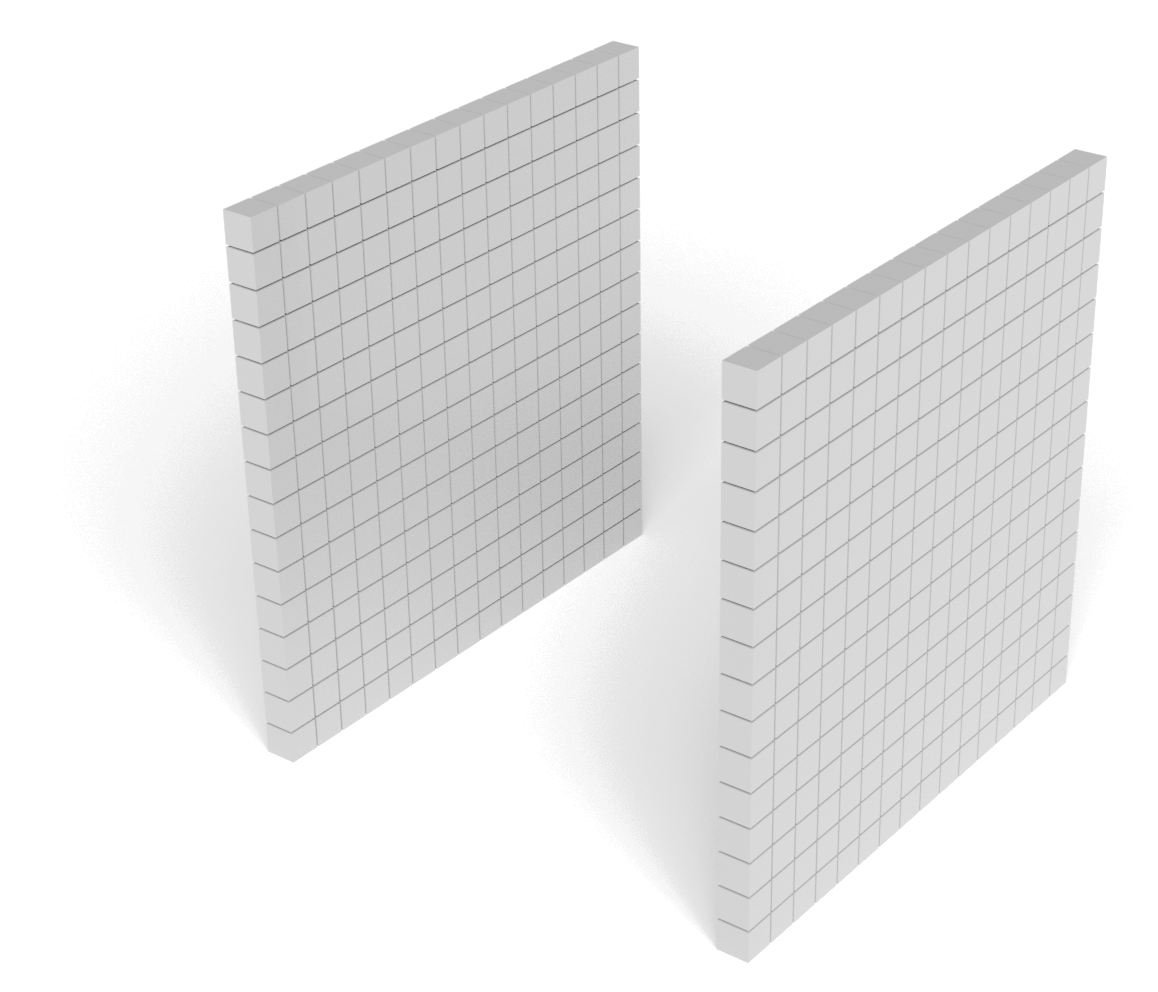
\includegraphics[width=\textwidth]{sections/methodology/figures/voxels-merge-1.png}
        \caption{Front side sample.}
        \label{fig:filling-non-watertight-model}
    \end{subfigure}
    \hfill
    \begin{subfigure}[t]{0.3\textwidth}
        \centering
        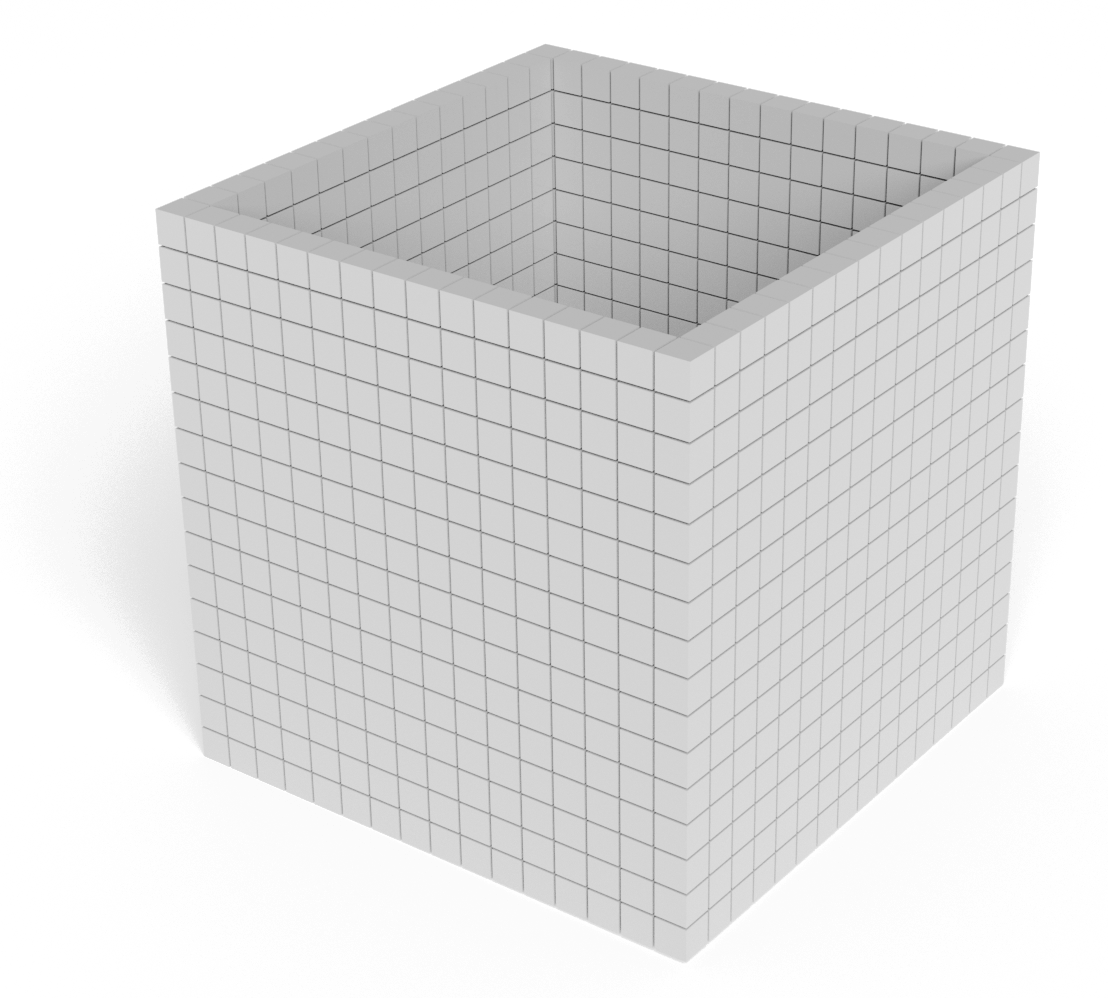
\includegraphics[width=\textwidth]{sections/methodology/figures/voxels-merge-2.png}
        \caption{Front and left side samples merged together.}
        \label{fig:filling-watertight-model}
    \end{subfigure}
    \hfill
    \begin{subfigure}[t]{0.3\textwidth}
        \centering
        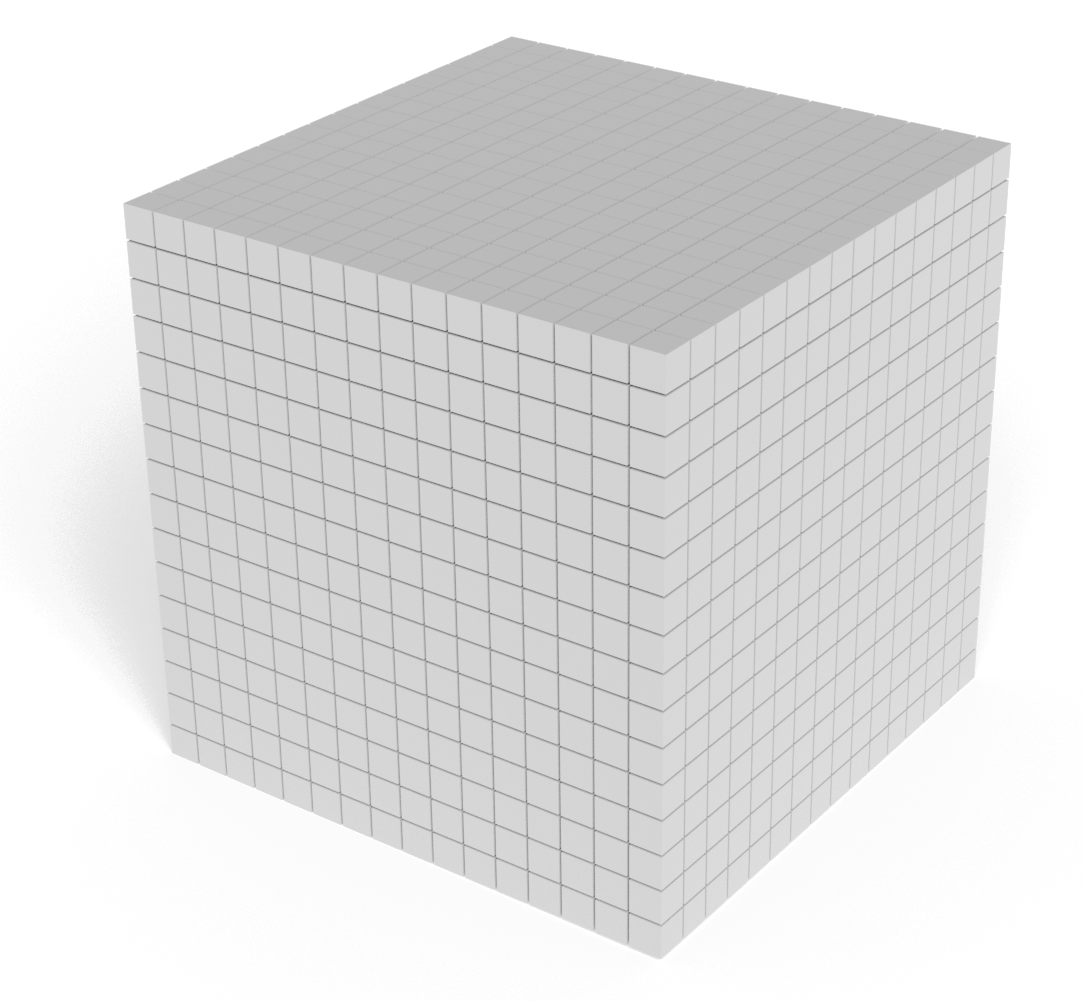
\includegraphics[width=\textwidth]{sections/methodology/figures/voxels-merge-3.png}
        \caption{Front, left and top side samples merged together.}
        \label{fig:filling-watertight-model}
    \end{subfigure}
       \caption{Merging of voxel samplings.}
       \label{fig:voxel-sample-merging}
\end{figure}

The algorithm also has an option for producing filled, or solid, results. This is achieved by interpreting the first raycast intersect as the surface of the object. From this point will everything be considered "inside" the object. When a second intersect is detected, the state is changed to be "outside" the object. A new hit would indicate "inside", and so on. This works very well with a watertight 3D model, as can be seen from figure \ref{fig:filling-non-watertight-model}. However, when trying to fill an object which is not watertight, this can result in severe inaccuracies. This can be seen in figure \ref{fig:filling-watertight-model}

\begin{figure}[h]
    \centering
    \begin{subfigure}[b]{0.45\textwidth}
        \centering
        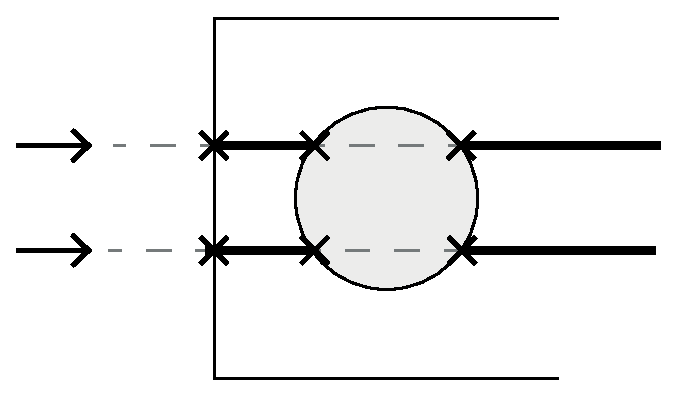
\includegraphics[width=\textwidth]{sections/methodology/figures/solid-non-watertight}
        \caption{Non-watertight 3D model cross section.}
        \label{fig:filling-non-watertight-model}
    \end{subfigure}
    \hfill
    \begin{subfigure}[b]{0.45\textwidth}
        \centering
        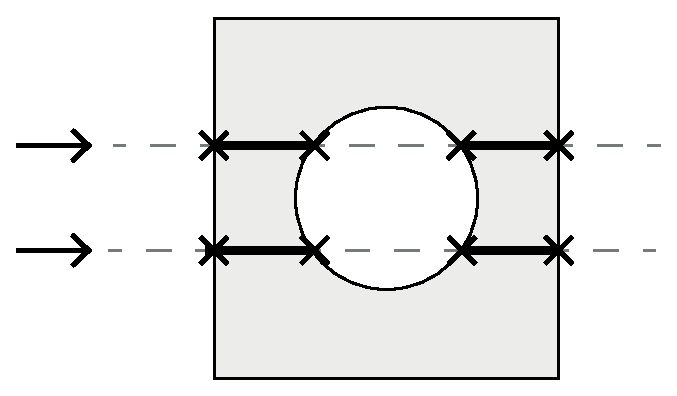
\includegraphics[width=\textwidth]{sections/methodology/figures/solid-watertight}
        \caption{Watertight 3D model cross section.}
        \label{fig:filling-watertight-model}
    \end{subfigure}
       \caption{Solid (voxelization) filling of 3D model cross section.}
       \label{fig:filling-3d-model}
\end{figure}

(\colorbox{RubineRed}{Remove watertight model?}) 

\subsection{three.js optimization}
The raycasting functionality, used by the raycasting algorithm described in Section \ref{sec:method-raycasting-algorithm}, is supplied by the three.js library. The library provides a throughly tested and accurate raycasting solution. However, it is CPU bound and  iterates every face of the mesh. This gives each raycasting operation a time complexity of O(n). If the 3D mesh is highly detailed, containing a large amount of polygons, the raycasting will take a long time to perform. After a careful assessment of potential solutions, the three.js plugin named three-bvh-mesh \cite{three-bvh-mesh} was used to improve this. This plugin provides a BVH implementation in order to speed up the raycasting against three.js meshes. By using this plugin, the time complexity for a single raycasting operation decreases from O(n) to O(log~n). Figure \ref{fig:bvh-monkey} shows an example visualization of a BVH tree applied to a 3D model, which is generated by the three-bvh-mesh plugin.

\begin{figure}[ht]
    \centering
    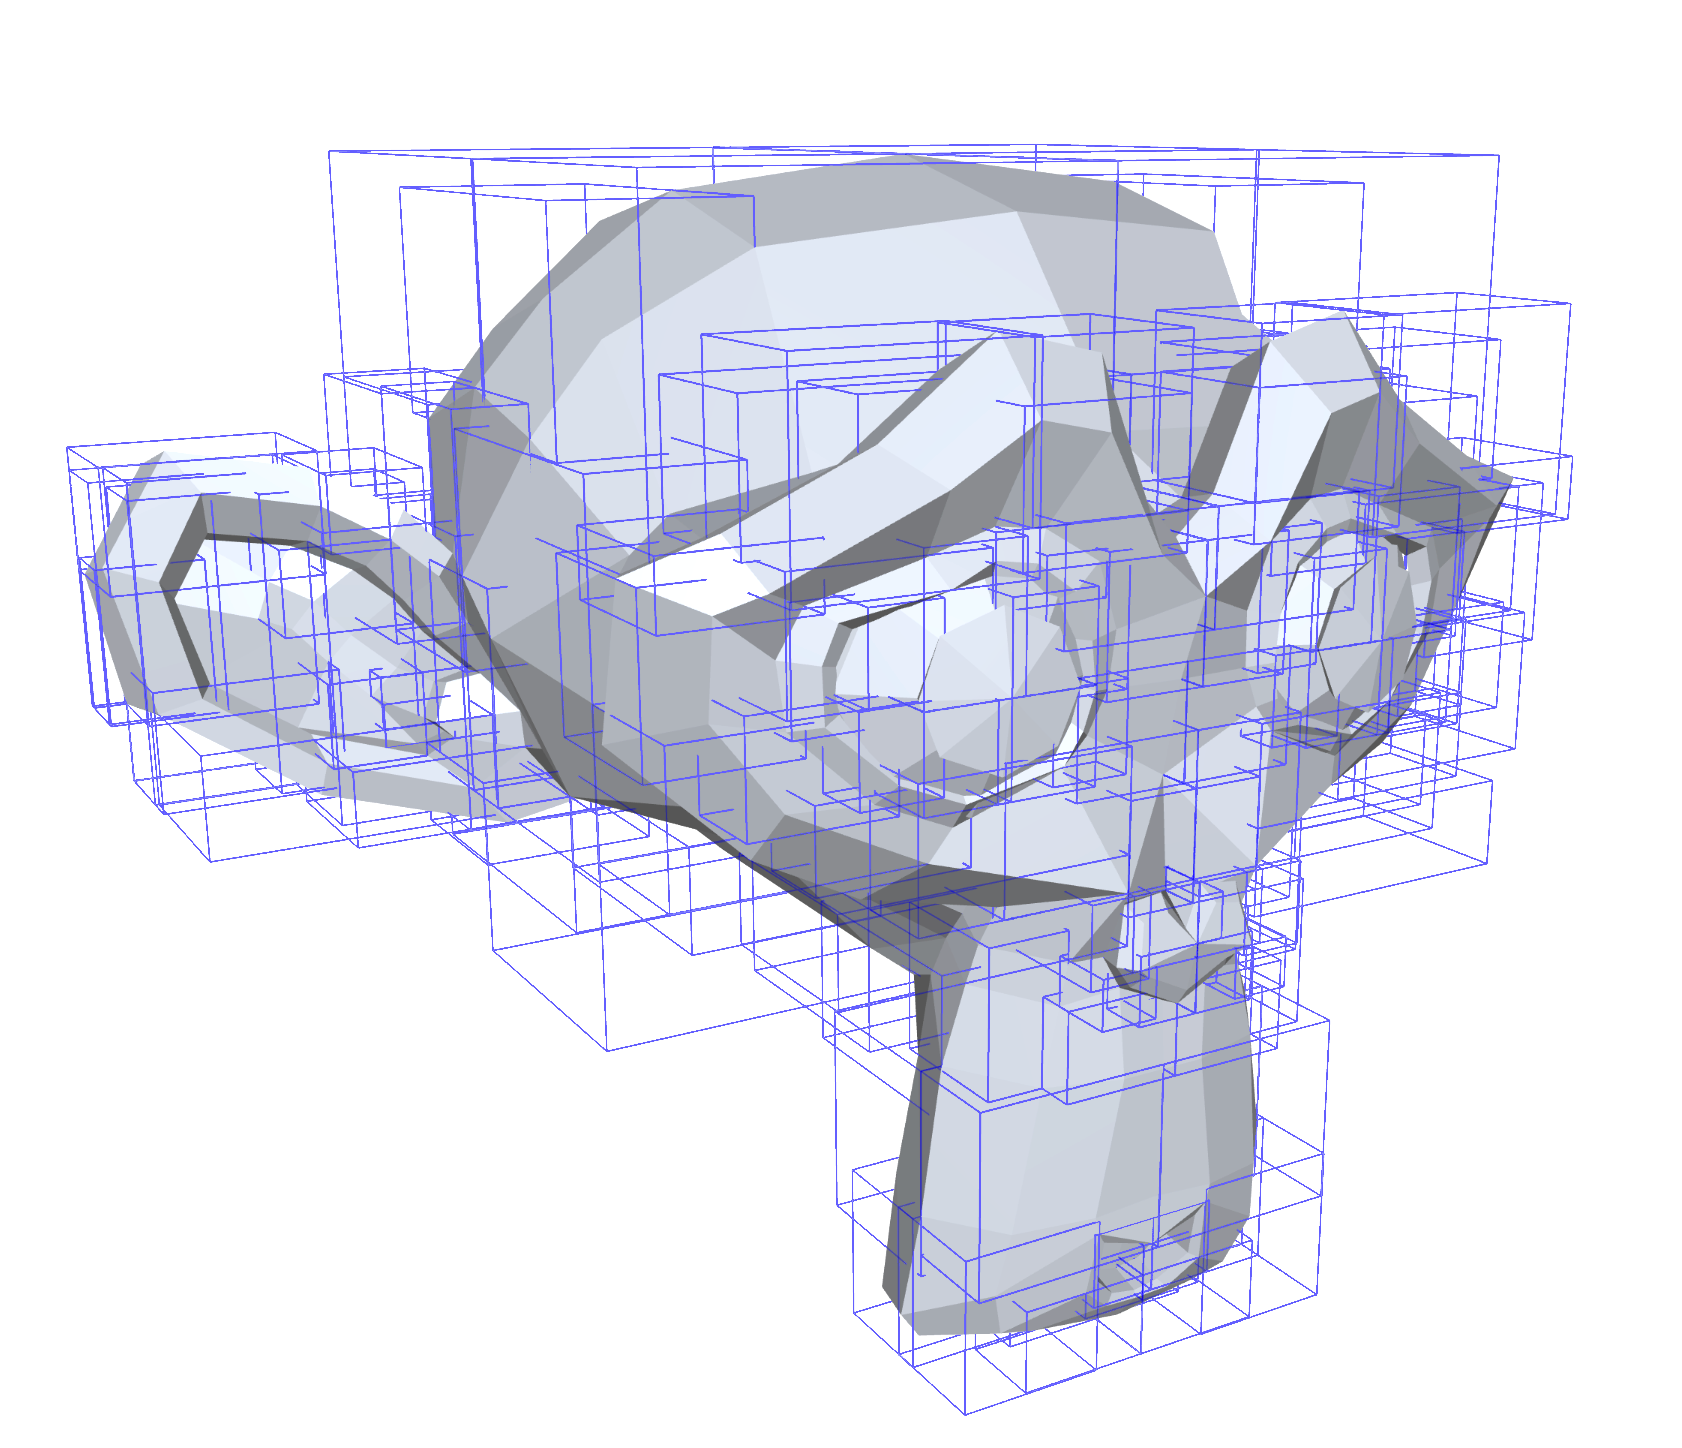
\includegraphics[width=0.5\textwidth]{sections/methodology/figures/bvh-monkey.png}
    \caption{Visualization of BVH applied to 3D model.}
    \label{fig:bvh-monkey}
\end{figure}

\subsection{Color system}
The color system of Voxelizer handles the storing and extraction of color from polygon meshes. This enables the engine to extract color information from the 3D mesh, and apply it to the voxels. The system mainly comprises of a ColorExtractor class and a TextureHandler class. The TextureHandler class stores a copy of all the texture maps associated with a 3D object. These are stored in a hashmap, using the texture maps UUID as key. Further, it is able to look up a UV coordinate of a texture map in its store, retrieving the corresponding color. See Section~\ref{sec:info-texture-maps} for more details on texture maps and UV coordinates. The ColorExtractor class provides various methods for extracting colors from from an raycast intersect. It uses the TextureHandler as internally texture storage, for fast lookup of texture colors. 

During raycasting with the raycasting algorithm described in Section~\ref{sec:method-raycasting-algorithm}, each intersect produces an UV coordinate of the associated texture map, along with its UUID. This info is then fed to a ColorExtractor class, returning the appropriate RGB color of the intersect. This color data is then stored in a four-dimensional view of a large ndarray. For maximum efficiency and safety, actual datatype supplied to ndarray is an Uint8ClampedArray~\cite{uint8clampedarray} (typed array).

\subsection{Loading}
The Voxelizer library/engine previously made use of a wrapper OBJ loader. This resulted in very limiting compatibility with other file formats. This support has been dropped in favor of the new ES6 JS loader modules introduced by three.js. three.js supports around 40 different file formats for loading 3D models. All three.js objects inherits from a base class named Object3D. This includes meshes. By ensuring compatibility with three.js meshes, any loader compatible with three.js can be used.

\subsection{Exporting}
As described in Section~\ref{sec:method-implementation}, the engine normally outputs ndarrays with color and voxel information, wrapped in a Volume class. However, the engine also comes with several exporter classes. This includes:
\begin{itemize}
    \item \textbf{XML} - XML provides a versatile and flexible file format. The native JavaScript DOM parser is used for the actual parsing of the XML data. The outputted format of the XML document structure is described on the GitHub wiki page for the engine.
    \colorbox{red}{PROVIDE LINK HERE !!!}
    \item \textbf{BINVOX} - BINVOX~\cite{binvox-file-format} is one of the more popular voxel data file formats. BINVOX is the file format used by the binvox~\cite{binvox} voxelization software. A separate repository named binvox~\cite{andstor-binvox} has been created for handling BINVOX files. See Section~\ref{sec:method-binvox}.
    \item \textbf{3D array} - An array exporter is implemented for exporting the voxel data as a normal nested JavaScript array. If the export includes color data, this is exported as a 4D JavaScript array.
\end{itemize}

\subsection{Testing}
Several unit tests are created for testing the different parts of the voxelization system. This ensures correct operation of the voxelization process, and protect against introducing new bugs. Jest~\cite{jest} has been chosen as the testing framework provider. Jest also provides coverage reports. These are very valuable in terms of analyzing what parts of the system is and is not tested.

\subsection{Migration}
The previous version of Voxelizer was version v0.1.3. Following Semantic Versioning~\cite{semantic-versioning}, or SemVer, the old version of Voxelizer is defined as still in Beta. Introducing a new Major version of the library with breaking functionality is therefore no problem. Still, a very simple migration guide is provided on the Wiki of the Voxelizer engine repository on GitHub \colorbox{red}{LINK HERE!!!!}.

\subsection{Debugging and Profiling}
During development, the three-voxel-loader plugin was used to visualize the actual voxel outputs. This made it easy to visually inspect the results of the voxelization algorithm. A similar solution to the debugging setup used for the three-voxel-loader plugin was used. Likewise, this also resulted in an example usage of the engine, and is deployed to GitHub Pages. \colorbox{red}{LINK TO VOXELIZER EXAMPLE PAGE}.

For assessing the memory consumption and speed of the engine, the performance tool~\cite{chrome-dev-tools-profiler} in the Google Chrome Developer Tools is used. This helped removing some CPU-heavy bugs, memory issues and other performance bottlenecks. Figure~\ref{fig:chrome-devtools-performance} shows an image of the performance tool.

\begin{figure}[ht]
    \centering
    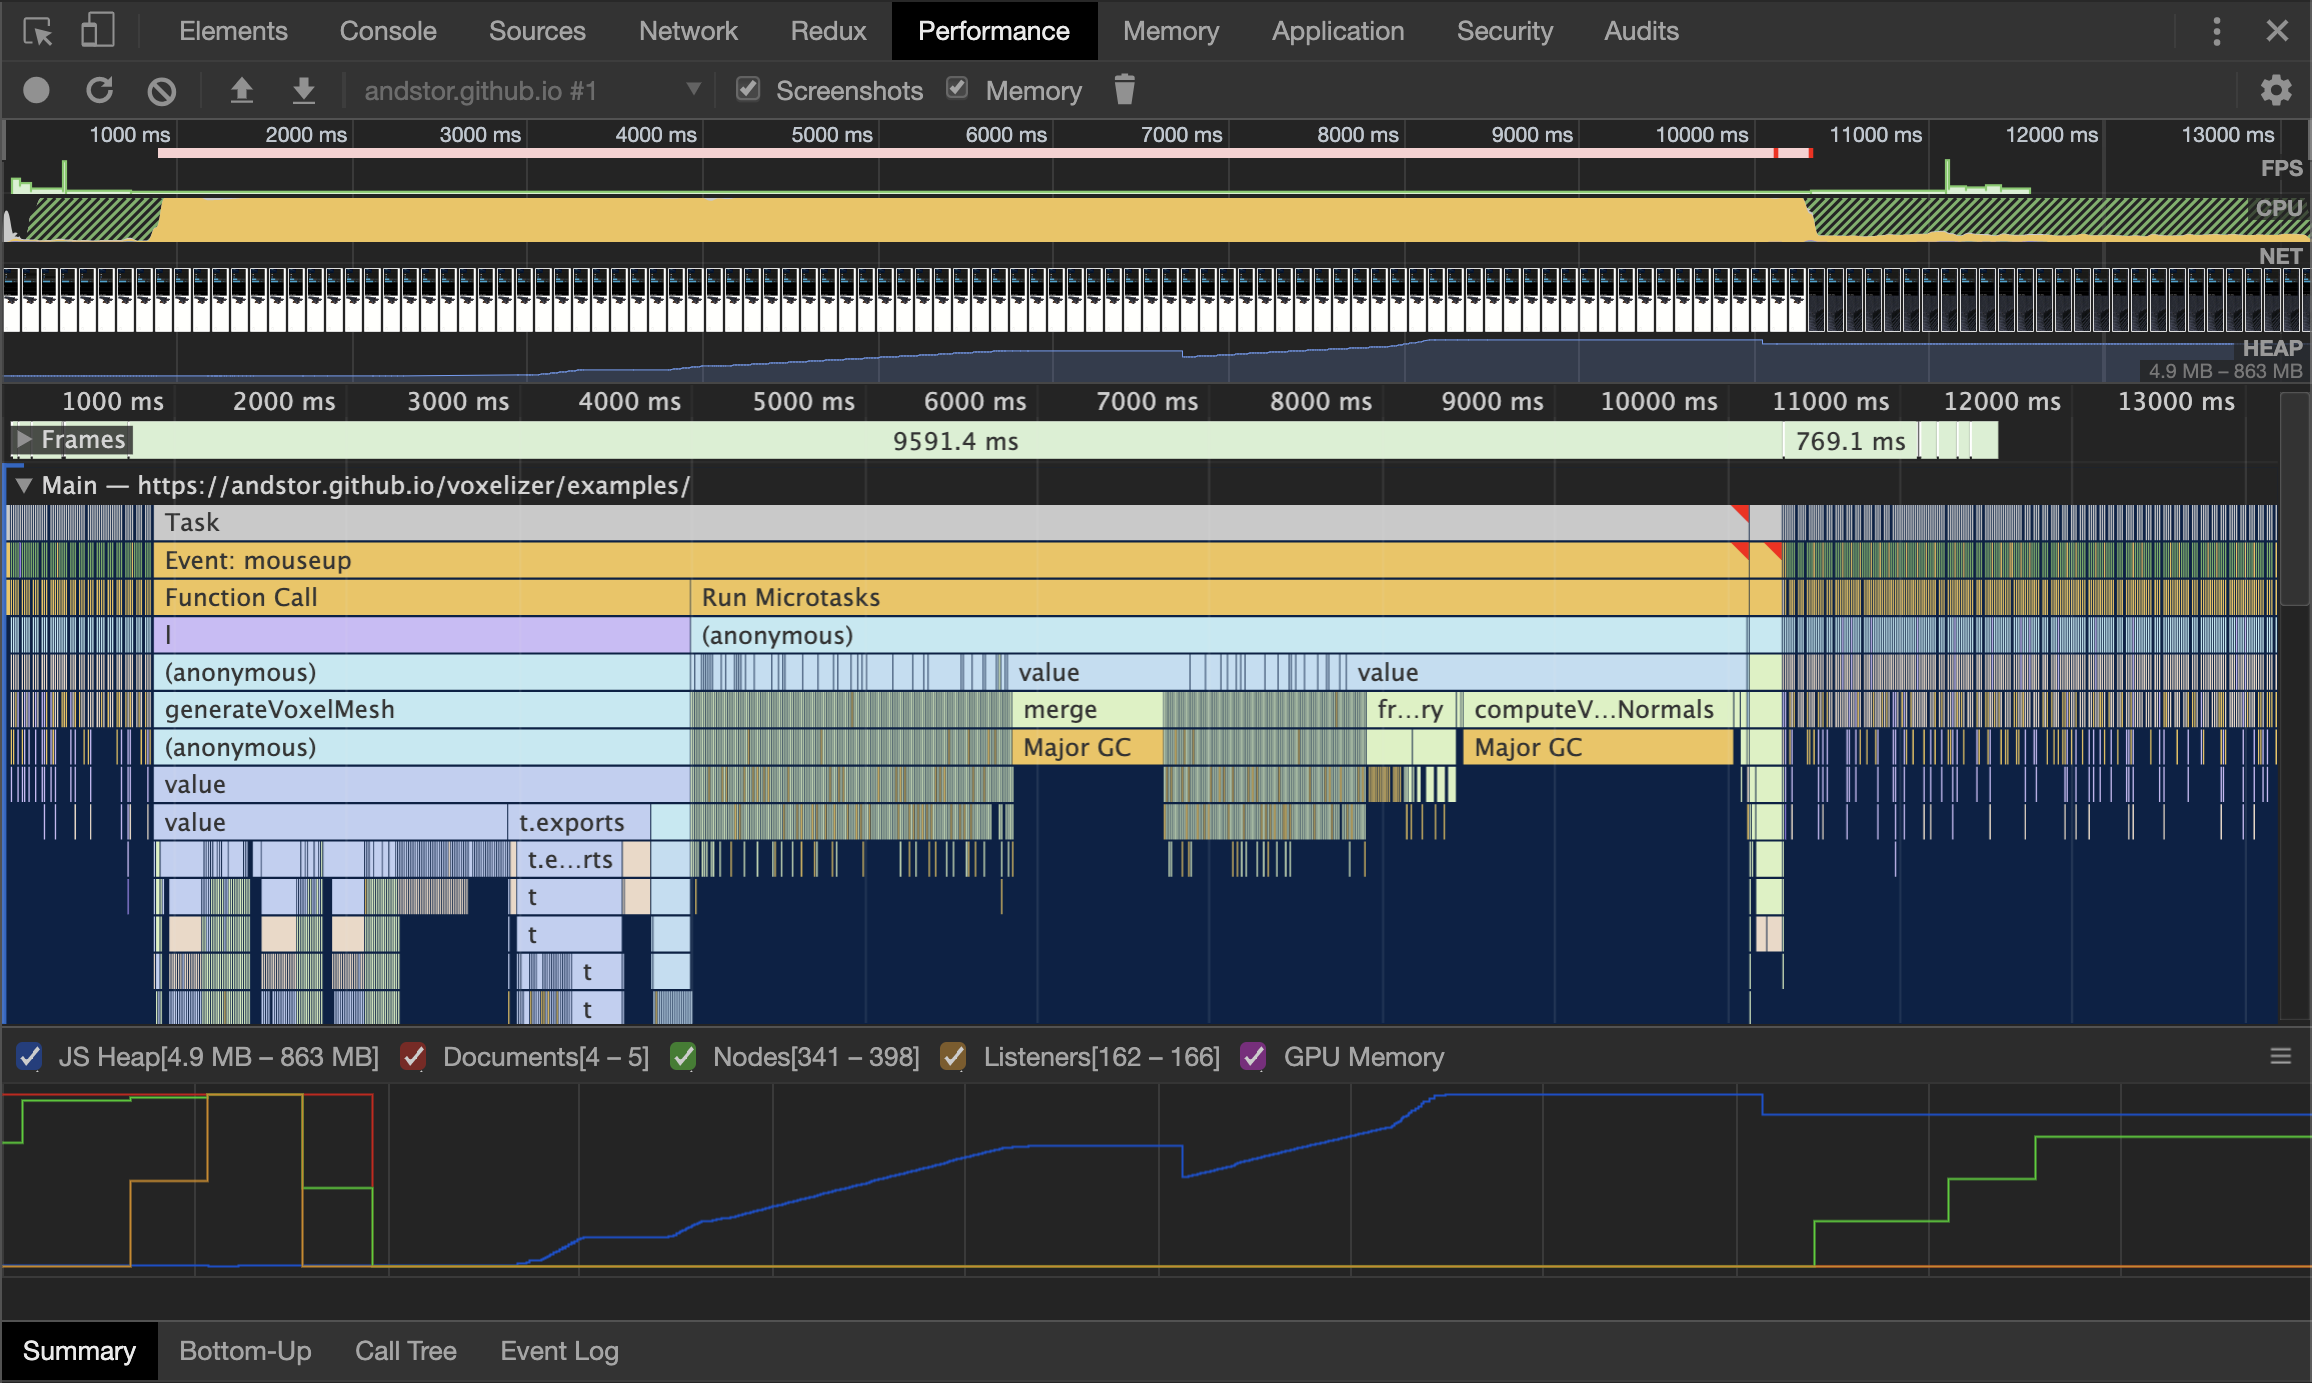
\includegraphics[width=\textwidth]{sections/methodology/figures/chrome-dev-tools-performance.png}
    \caption{Screenshot of performance profiling with Google Chrome Developer Tools.}
    \label{fig:chrome-devtools-performance}
\end{figure}

\subsection{Building}
The engine is bundled with Webpack. This gives great control over the building process. See Section~\ref{sec:theory-bundling} for more details on Webpack. Voxelizer also makes use of ES6 features, so all source files are also transpiled to ES5 with babel. The main output of the library is UMD, as described in Section~\ref{sec:theory-module-system}. This makes the engine compatible with a range of other module systems. However, since Webpack does not support ES Modules right out of the box, a better alternative would be to use Rollup \ref{sec:theory-bundling}. Unfortunately, this was not possible due to a circular dependency in one of the dependencies of Voxelizer. Therefore, in order to use Voxelizer as a native ES Module, a project also needs to use a module loader like Webpack.

\section{BINVOX}
\label{sec:method-binvox}
A separate open-source repo for building and parsing BINVOX file formats were created during refactoring of the Voxelizer engine and the three-voxel-loader plugin. It is named binvox and licensed under the MIT license. The BINVOX file format consists of a header in plain ASCII, followed by binary data. The binary data is compressed using run-length encoding. From the BINVOX specification: \textquote[\citet{binvox-file-format}]{The binary data consists of pairs of bytes. The first byte of each pair is the value byte and is either 0 or 1 (1 signifies the presence of a voxel). The second byte is the count byte and specifies how many times the preceding voxel value should be repeated (so obviously the minimum count is 1, and the maximum is 255).}.

The new binvox package provides tools to both parse and construct files according to the BINVOX file specification~\cite{binvox-file-format}. Parsing is done on the individual set of two bits, uncompressing the data and storing it in a JSON format. An example of the parsed JSON result can be seen in Program~Code~\ref{lst:binvox-example}. Similarly, a user can supply the same JSON data structure for constructing a BINVOX file resource. Hence, parsing and building commute.
\lstinputlisting[language=JSON,style=numbers,label={lst:binvox-example},caption={Example BINVOX data in JSON format}]{sections/methodology/code/binvox-json.json}

\section{Voxelizer-Desktop}
\colorbox{red}{WRITE THIS SECTION!!!!}
\subsection{Electron}
\subsubsection{Auto updating}

\subsection{GUI}
... Sketches?? Wireframe diagrams of GUI etc...


\section{JSDoc Action}
In the next couple of subsections, the implementation and design decisions of the JSDoc Action will be presented.
\subsection{Implementation}
For creating a GitHub Action, several mandatory files and configurations has to be created. This documentation is available at GitHub. GitHub Actions provides two main types of action. One is JavaScript based. The other is based on Docker. They both have their advantages and disadvantages. A Docker container action provides an isolated environment, providing extremely flexible and stabile solutions. However, it is only possible to run on Linux. On the other hand, a JavaScript GitHub Action can be run directly on a runner machine. This makes it a lot faster than a Docker based Action. This is because of latency due to retrieve and build the container. A JavaScript action is also cross platform compatible, meaning it can run on both a Linux, Windows or MacOS operating system. In order to provide a fast and cross compatible solution, the JavaScript action type is chosen for the JSDoc Action.

The JSDoc Action is made up of mainly two parts. One is the template installation system, and the other is the actual execution of the JSDoc tool. For providing maximum flexibility, all functions of the JSDoc tool is made available as input configurations through the GitHub Actions Workflow API. The action is also able to use a JSDoc configuration file \cite{jsdoc-config-file}. If a user provides a template to be installed, the action will first install this. This is done with the help of the node package manager (npm). The supplied template can be everything from a GitHub repository, to an npm package. The installed template files are then processed. The action does all of its IO operations asynchronously, ensuring fast execution speed of the action. When finished, a JSDoc CLI command is then formed based on the various user inputs and (if provided) config file. This command is then executed, effectively telling JSDoc to generate the documentation. The result is a user defined output folder with the generated API documentation.

\subsection{Usage}
For actually using the action in a Workflow, the action makes a couple of assumptions. Firstly, the actual source files to generated documentation from needs to be supplied. This is normally solved by using the Checkout~Action~\cite{checkout-action} made by GitHub. Secondly, the JSDoc Action only generates an output directory with files. This means that nearly any deployment action can be used for upload the files the desired service, for example GitHub pages. The deployment action supplied as example in the README.md file of the repository is named GitHub~Pages~Action~\cite{github-pages-action}.

\subsection{Feedback}
The JSDoc Action generated quite a lot of feedback from eager users of the action. Several wanted to test the action, and multiple issues were filed in the issue tracker on GitHub~\cite{jsdoc-action-issue-tracker}. See for example issue~\#20~\cite{jsdoc-issue-20}. Since maintenance is essential to the success of an open-source project, all feedback were responded to and handled accordingly. Alongside the development of the other main projects, many bug-fixes were made to the JSDoc Action. Eventually, all issues were resolved, resulting in several happy users.


\section{Automation}
Automation is an important part for ensuring both efficiency and security. The next subsections will contain a description of how the various open-source systems developed in connection with this thesis have been automated.

\subsection{JavaScript package workflows}
\label{sec:method-javascript-package-workflows}
GitHub provides CI and CD as a part of its GitHub Actions system. This system has been put to use, creating several workflows in order to automate various tasks like testing, building, documentation generation and publishing. The workflows have been made so that they should work out of the box for similar projects. See Section~\ref{sec:theory-github-actions} for a description of GitHub Actions. Do note that the default behavior of Workflows is to terminate if any errors are encountered.

Figure~\ref{fig:cicd-pipelines} shows a simplified diagram of the CI/CD automation pipelines created for the JavaScript packages which are to run on new contributions to the codebase. This system mainly consists of two workflows. One for building the package, and one for generating and publishing API documentation. A simple step by step walkthrough of the system is now presented.

\begin{enumerate}
    \item \textbf{Pull request} - The pipelines are mainly triggered by a pull request. This starts up both a security analysis by LGTM and a build workflow.
    \item \textbf{Security analysis} - As described in Section~\ref{sec:theory-semmle-lgtm}, LGTM provides a security analysis. If any vulnerabilities are found, the pull request fails.
    \item \textbf{Build workflow} - The build workflow has four steps.
    \begin{enumerate}
        \item \textbf{Checkout} - First, the repository in which the automation is done on is cloned.
        \item \textbf{Build} - Then, the JavaScript project is built.
        \item \textbf{Test} - If the project provides tests, these are also run.
        \item \textbf{Coverage} - Coverage reports are created with Jest.
    \end{enumerate}
    \item \textbf{Coveralls} - The coverage report is then published to Coveralls.io. See Section~\ref{sec:theory-coveralls} for details on Coveralls.
\end{enumerate}

If the workflow finishes, the security analysis comes out clear, and the coverage percentage is not decreased, the pull request is approved for merging. When a user with the appropriate privileges approves the pull request, the code is merged into the base branch. If the base branch is the master branch, a second workflow is started. This is a workflow for generating/updating the API documentation.

\begin{enumerate}
    \item \textbf{Checkout} - The source repo is cloned once again.
    \item \textbf{JSDoc Action} - The JSDoc Action is then used for generating JSDoc API documentation.
    \item \textbf{GitHub Pages} - The outputted documentation is then finally deployed to GitHub Pages with an action called \cite{github-pages-action}.
\end{enumerate}

\begin{figure}[hp!]
    \setlength{\abovecaptionskip}{25pt}
    \centering
    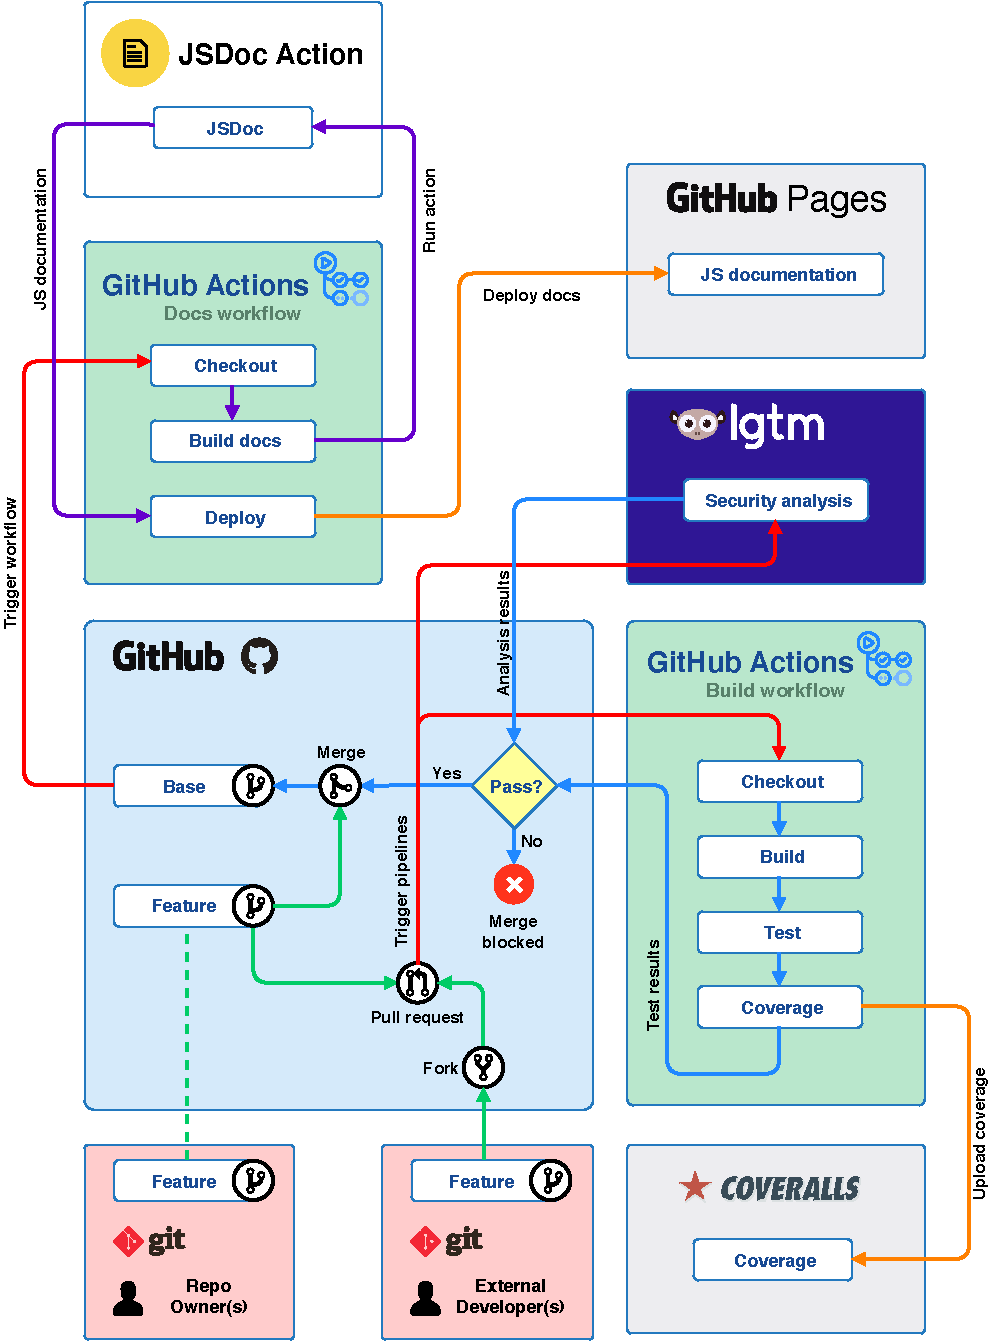
\includegraphics[page=1,scale=1]{sections/methodology/figures/pipelines.pdf}
    \caption{CI/CD pipelines}
    \label{fig:cicd-pipelines}
\end{figure}
%\clearpage

In order to automate the release process of a JavaScript package, a third workflow is used. This is shown in Figure~\ref{fig:release-automation}. It mainly involves packaging and publication of the software to the npm~registry~\cite{npm-registry}. The workflow functions like this:
\begin{enumerate}
    \item \textbf{Trigger release} - First, a user with the appropriate privileges needs to create a release manually on GitHub. This generates a git tag. Further, the release starts up the package workflow.
    \item \textbf{Package workflow}
    \item \begin{enumerate}
        \item \textbf{Checkout} - The source repo is cloned once again.
        \item \textbf{Build} - The JavaScript project is then built.
        \item \textbf{Test} - If the project provides tests, these are also run.
        \item \textbf{Package} - If all the above tests are completed without errors, the project is then packaged.
    \end{enumerate}
    \item \textbf{Publish package} - If the package workflow completes, the new package is then published to the npm registry.
\end{enumerate}

\begin{figure}[hp]
    \setlength{\abovecaptionskip}{25pt}
    \centering
    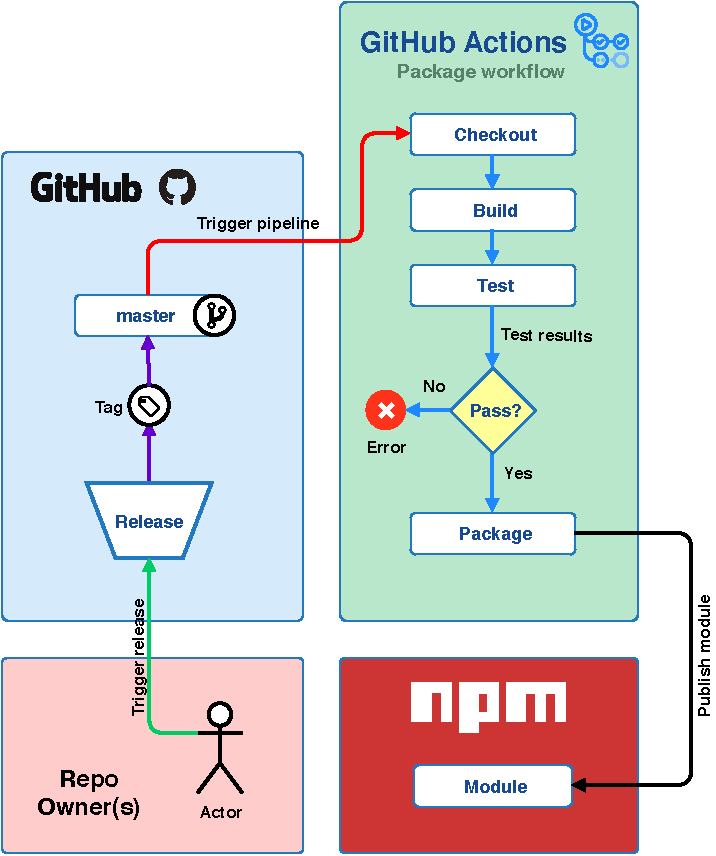
\includegraphics[page=1,scale=1]{sections/methodology/figures/package-release-automation.pdf}
    \caption{Automation of release publishing process.}
    \label{fig:release-automation}
\end{figure}

\subsection{GitHub Action version tagging}
GitHub provides guidelines in terms of versioning and tagging of a GitHub Actions \cite{github-actions-versioning}. According to Github, releases should be following Semantic Versioning. When a new release is made, the major tag (v1, v2, etc.) should be moved to point on the Git ref of the current release. This process is tedious. A workflow has therefore been created for automating this release process. Figure~\ref{fig:update-major-tag} provides an illustration of the moving of Git tags. An action named actions-tagger~\cite{actions-tagger} already provides support for this tagging scheme.

Following
Auto major version tagging update

\begin{figure}[hp]
    \setlength{\abovecaptionskip}{25pt}
    \centering
    \hspace*{-2cm}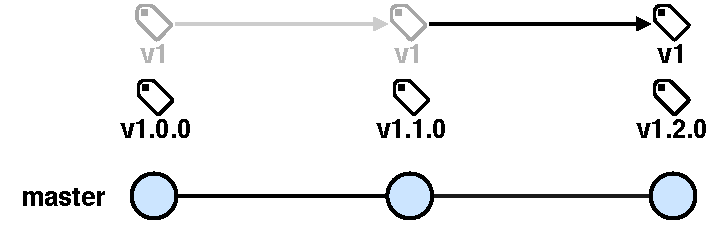
\includegraphics[page=1,scale=1]{sections/methodology/figures/update-major-tag.pdf}
    \caption{Automatic updating of major version tag.}
    \label{fig:update-major-tag}
\end{figure}

\section{file-existence-action}
\label{sec:method-file-existence-action}
In order to be able to produce the general purpose workflows described in Section~\ref{sec:method-javascript-package-workflows}, it became apparent that i needed to be able to check if a file existed. Normally, a coverage script is defined in the projects package.json file. This runs all the tests and produces a coverage report file. However, if no such script is provided, the workflow will run the tests manually instead, and no file will be generated. If no such file is generated, this needs to be detected by the workflow, in order to avoid running the upload to Coveralls.io step. This resulted in a relatively small GitHub Action, named File Existence. The action is written in TypeScript, and based on a template provided by GitHub. The action is able to check one or more paths for the existence of a file. The boolean result is then available to the following steps in the workflow.

\section{file-reader-action}
Following the problems described in Section~\ref{sec:method-file-existence-action} above, another problem arises if the coverage script is defined, but no tests are created. If this is the case, an empty coverage file is created. Trying to upload this to Coveralls.io results in an error. The need for reading the contents of a file was therefore necessary, in order to check if the coverage file is empty. If it is empty, the Coveralls step should not be executed. The solution was to create a small GitHub Action, named File Reader. The action is written in TypeScript, and based on a template provided by GitHub. The action is able to read the contents of a file path supplied by the user. THe output is then available to the consequently workflow steps.